
The case for software development is the same as with requirements engineering: Design Science Research has little guidance.
And again, the software engineering field has the answers.\\

The goal for the development methodology is to \textbf{create the right solution}, which solves the identified problem and fulfils the software requirements.
The methodology also aims to \textbf{avoid or reduce risks} for project failure, by tackling it as early as possible.
Research often deviates from routine design here, by going for the risks first instead of delaying or hiding them, as this may lead to new knowledge~\cite[p.~114]{oatesResearchingInformationSystems2006}.\\

Another goal for the development process is to create ``good'', high quality software, so the project can be accepted by the \gls{open source} developer ecosystem for further development and maintenance.
Bad code or a bad design may result in a full rewrite by the next interested developer, or the developer may try to contribute but find it hard and give up.\\

Development methodology will not follow one strict practice, but rather piece together many different practices and values, which have lead to good results in the author's past.


\subsection{Agile}

Development will follow agile values and principles, as described in \citetitle{kentbeckManifestoAgileSoftware2001}~\cite{kentbeckManifestoAgileSoftware2001} and \citetitle{PrinciplesAgileManifesto}~\cite{PrinciplesAgileManifesto}.
This means readjusting plans, rapid feedback from stakeholders, and software that works underway in development.

\paragraph{Agile development}
As there are many unknown factors in development, such as third party components and services to comply and integrate with, and unknown and hard to use \glspl{API}, the plans and designs may change.
As with software requirements, the data structures, algorithms and design in the software solution will have to change as the developer learns the systems and problem space better.
\textbf{Responding to change} will be valued more than following a plan here.
Also, \textbf{working software} is more valuable than extensive documentation, meaning that code comments, tests, design specifications and diagrams will be given less effort than code, particularly if done up-front before the code.
The alternative is that this documentation is made, but the code for it quickly proves itself impossible to make, or there is not enough time to implement it, leaving only useless documentation as the result.
This also ties in to \textbf{simplicity and maximizing work-not-done}.\\

Regular reflection will be used weekly or bi-weekly, to assess if the process can be more effective.
Sometimes tools and technologies may seem like a good fit for the development, but instead wastes more time than the developer productivity provided.
Retrospective analysis of the development progress will try to detect this, and then expose if bad approaches are used.
If so, these will be removed or replaced if possible.\\

Stakeholder involvement is important as well.
The development will have a stakeholder as the developer (the author), which knows how the artifact will be used.
Additionally, the supervisor will see a demo during development, to provide feedback and help prioritize the next steps.


\subsection{Iterative Development}

The software system will be developed iteratively.
This means the components will be implemented up to a threshold of functionality, and executed to evaluate the behavior.
The evaluation is not a formal and rigorous one, but rather informal and aims to quickly confirm if the software has the correct behavior.
Then the components are developed some more, in a loop until the project ends.\\

The components are also developed incrementally.
It also means a component will be worked on until it reaches \textit{some} functionality, and then the next component will be worked on until it is on par.
No component is developed to completion while the others are not started on.


\subsection{Lean and Minimum Viable Product}

Lean development is a set of principles inspired from Lean Manufacturing (for automobiles and such)~\cite{rachellelynnGuidingPrinciplesLean}.


\paragraph{Eliminate waste}
A core principle is to \textbf{eliminate waste}.
This is also seen in Agile, as maximizing work-not-done.
What Lean regards as waste is any work and output that does not have value.
This means avoiding: unnecessary code and functionality (things deemed ``could be nice to have''), unfinished work in progress (code and features not completed), defects and poor quality (do it well, do it once).


\paragraph{Build quality in}
Another principle is \textbf{building quality in}.
Important business logic should have automated unit tests (however not all code needs tests\footnote{A project with high uncertainty and changing requirements may find tests a hinder as they have to up updated all the time. This results in extra work and rework.})
Tedious and repetitive tasks should be automated, for example with scripts and tools.


\paragraph{Create knowledge}
A third principle is to \textbf{create knowledge}.
Code will have comments where needed\footnote{Not all comments are good comments. Code with side effects, strange design choices or hard to read implementation may need clarification by using comments.}.
Documentation will explain the software at a high level.


\paragraph{Deliver fast}
The last principle applied is to \textbf{deliver fast}.
While there are no students to use the artifact now, the focus is still on creating a functioning solution as early as possible.
This is done by prioritizing the requirements in an order to get a \textit{minimum viable product} (MVP).
This is a solution that is just barely usable.
The goal is to get it into the hands of users as quickly as possible, because this creates valuable feedback.

\subsection{Tracer Bullets}

\paragraph{Tracer bullets}
Using Tracer Bullets in code is a metaphor from \citetitle{huntPragmaticProgrammerJourneyman2000}~\cite{huntPragmaticProgrammerJourneyman2000}.
When using a machine gun, the operator does not precisely calculate where to shoot ahead of time.
Instead, tracer bullets are occasionally loaded into the gun, which glow up and give visual feedback to the operator as to where the bullets travel.


\paragraph{Tracer code}
The same idea applied to coding means that uncertainty and risk is not dealt with by heavy upfront planning.
A software solution likely has to interface with many unknown parts, adding risk for each one.
The developer creates ``tracer code'', which has the goal of quickly connecting all the components and parts of the system, without adding lots of functionality.
Stubs and empty code can be used so the code compiles, as long as all the actual components in the final design are integrated and running.
If any problems are discovered, then adjust and redesign as necessary~\cite{huntPragmaticProgrammerJourneyman2000}.\\

The tracer code is real code, not a prototype.
Therefore, it should be made with proper quality.
It just lacks functionality.
With a working skeleton system, more functionality can be added on top.


\subsection{Domain-Driven Design}\label{sec:ddd}

Domain-driven design is an approach to domain modeling in software.
The goal is to create a domain model in software that uses the same language a domain expert uses, to create better, more evolvable and understandable code.
If the domain has for example ``trees'' and ``nodes'', the code will also use trees and nodes as names, making stakeholder discussion straight forward.
The code will accurately model the domain, increasing understanding and capturing the details of the business logic~\cite{evansDomaindrivenDesignTackling2004}.
The model is represented as normal, executable code.
There is no specific file representation, and no \acrshort{MDD} framework involved.
This is not a \acrshort{MDD} method --- it is a object oriented coding and naming method.\

Another element from Domain-driven design is to use a layered software architecture.
The domain model is isolated from the rest of the code.
This makes it easy to see and reason about the behavior of the code, in terms of business logic~\cite[p.~69]{evansDomaindrivenDesignTackling2004}.
The alternative is that business logic is spread around the system, partially in the user interface components, persistence logic, and so on.
The layers makes every aspect of the program more cohesive and makes interpretation of the designs easier~\cite[p.~69]{evansDomaindrivenDesignTackling2004}.\\

Practically, the domain model will be in its own layer, and the user interface will be in its own layer.
The user interface will depend on the domain model.
The domain model will be unaware of any user interface.
An illustration is shown in \cref{fig:ddd-layered}.

\begin{figure}[htbp]  % order of priority: h here, t top, b bottom, p page
  \centering
  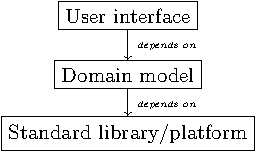
\includegraphics{figures/layered.pdf}
  \caption[Layered Architecture]{\textbf{Layered architecture}. The components above depends on the components below, but not vice versa.}\label{fig:ddd-layered}
\end{figure}


\subsection{Test-Driven Development}
%TODO

Test-driven development is about creating automated tests before writing the implementation~\cite[p.~105]{knibergScrumXPTrenches2015}.
It will be used sparingly, for cases where the behavior is complex and important to get right.
The developer will have to judge when it is needed, based on expected complexity, requirements and behavior for a unit of code.
This may be especially relevant for some business logic in the domain model.
Writing the tests first also creates a more testable design~\cite[p.~106]{knibergScrumXPTrenches2015}.\\

The benefit of automated tests is confidence in the code against bugs.
It also helps for when other developers join the project, as they can be confident about making changes without breaking existing code.
A goal is to have other contributors develop this project further, and therefore avoiding ``legacy code'' is a good thing.
The author of \citetitle{feathersWorkingEffectivelyLegacy2005} writes:

\begin{quotation}
``Legacy code is somebody else’s code. But in programmer-speak, the term means much more than that. 
[\ldots]


In the industry, \textit{legacy code} is often used as a slang term for difficult-to-change code that we don’t understand. 
[\ldots]


To me, \textit{legacy code} is simply code without tests. [\ldots]


Code without tests is bad code. It doesn’t matter how well written it is; it doesn’t matter how pretty or object-oriented or well-encapsulated it is. With tests, we can change the behavior of our code quickly and verifiably. Without them, we really don’t know if our code is getting better or worse.''


---~\textcite{feathersWorkingEffectivelyLegacy2005}
\end{quotation}


\subsection{Prototyping}

Prototyping will be used to create simple implementations when there is uncertainty of the design and big risks.
A prototype will create learning by coding in the real environment, and then prototype code is discarded afterwards.
A prototype can test feasibility and reveal good and bad sides of a design, quickly and cheaply.\\

The main bulk of prototyping has already been performed, as part of the pre-project in \cite{rekstadModelingEnvironmentCloud2020}.
